\section{Out-of-sample forecasting and economic value}\label{sec:forecast}

\subsection{Design}

\paragraph{Target and walk-forward.} The target is the four-hour log return
$y_{t}=\log C_{t+4}-\log C_t$, formed at the close of hour $t$. The first six months after the
feature warm-up are used only for training. The remaining sample (\BTCoosStart{} to \BTCoosEnd,
\BTCnOOS{} hours) is cut into \BTCnFoldsWF{} consecutive 30-day test blocks. Before each block every
model is re-estimated on all observations whose label is observable at the block start, i.e.\ with
$t+4$ strictly before the block (purging); nothing from the block enters estimation. Within each
training window the last 20\% serves as a validation block, itself purged from the inner training
rows, on which hyper-parameters are chosen before the model is refitted on the full window.
Winsorisation bounds (1st and 99th percentiles) and standardisation moments are estimated on the
training window only. Automated tests replace every bar after $t$ by noise and verify that features
at $t$ are unchanged, and check the purge condition for every fold (Appendix~\ref{app:leakage}).

\paragraph{Models.} Following \citet{gu2020}, models forecast the return relative to zero. The
elastic net is fitted without intercept on standardised features, with the penalty chosen from a
13-point grid and the $\ell_1$ share from $\{0.1,0.5,0.9\}$ on the validation block. As a non-linear
benchmark we use gradient-boosted trees with depth three, at least 300 observations per leaf and a
learning rate of 0.03, with the number of rounds chosen on the validation block. We also report the
historical-mean forecast. We estimate every model on every feature set defined in
Section~\ref{sec:measures} and report all of them.

\paragraph{Statistical evaluation.} The out-of-sample $R^2$ relative to a benchmark $b$ is
$R^2_{OOS}=1-\sum(y-\hat y)^2/\sum(y-\hat y^{b})^2$ \citep{campbell2008}. Because the zero forecast and
smaller feature sets are nested in larger ones, we test equal predictive accuracy with the
\citet{clark2007} statistic (one-sided), which adjusts for the noise that estimating irrelevant
parameters adds to the larger model, and report the \citet{diebold1995} statistic, which compares
realised accuracy. Overlapping four-hour targets make forecast errors serially correlated, so all
$t$-statistics use \citet{newey1987} standard errors with $\max(24,2h)$ lags. The information
coefficient (rank correlation of forecast and outcome) is reported with a 95\% moving-block bootstrap
interval with 48-hour blocks \citep{kunsch1989}.

\paragraph{Economic evaluation.} Each hour a signal $s_t\in\{-1,0,1\}$ is formed and held for four
hours with a quarter of capital per sleeve \citep{jegadeesh1993}, so the position over $(t,t+1]$ is
$\frac14\sum_{k=0}^{3}s_{t-k}$; every forecast is used and no exposure is double counted. The
\emph{sign} rule sets $s_t=\operatorname{sign}(\hat y_t)$, which is zero when the model predicts
exactly zero; the \emph{selective} rule trades only when $|\hat y_t|$ exceeds the 80th percentile of
the model's absolute in-sample forecasts in the current training window. Costs of
$c\in\{0,2,5,10\}$ basis points are charged per unit change in position. We report the break-even cost
at which net profit is zero, the HAC $t$-statistic of the intercept in a regression of strategy
returns on BTC returns, the number of calendar years with a positive Sharpe ratio, and the deflated
Sharpe ratio (DSR) of \citet{bailey2014}. The DSR is the probability that a strategy's true Sharpe ratio
exceeds the maximum expected among all \BTCnTrials{} model and rule combinations under the null of no
skill, given their dispersion, the sample length and the non-normality of returns.

\subsection{Forecast accuracy}

\begin{table}[t]
\centering\caption{Out-of-sample forecast accuracy, four-hour BTC/USDT returns}\label{tab:forecast}
\resizebox{\textwidth}{!}{\begin{tabular}{lrrrrcrr}
\toprule
Model & $R^2_{OOS}$ vs.\ 0 (\%) & $R^2_{OOS}$ vs.\ mean (\%) & CW $t$ vs.\ 0 & IC & 95\% CI & Hit rate & Hit $t$\\
\midrule
Historical mean & \ensuremath{-}0.075 & 0.000 & -- & \ensuremath{-}0.002 & [\ensuremath{-}0.021, 0.015] & -- & --\\
EN: TI & \ensuremath{-}0.055 & 0.020 & 1.40$^{*}$ & 0.002 & [\ensuremath{-}0.014, 0.019] & 0.491 & \ensuremath{-}2.14\\
EN: MS$_{\text{proxy}}$ & \ensuremath{-}0.139 & \ensuremath{-}0.064 & \ensuremath{-}0.61$$ & \ensuremath{-}0.005 & [\ensuremath{-}0.024, 0.013] & 0.488 & \ensuremath{-}2.05\\
EN: MS & \ensuremath{-}0.006 & 0.070 & 0.86$$ & \ensuremath{-}0.002 & [\ensuremath{-}0.019, 0.014] & 0.494 & \ensuremath{-}0.92\\
EN: ALL & \ensuremath{-}0.025 & 0.050 & 1.34$^{*}$ & 0.019 & [0.004, 0.035] & 0.508 & 1.44\\
EN: Flow$_{\text{BVC}}$ & \ensuremath{-}0.081 & \ensuremath{-}0.005 & \ensuremath{-}1.35$$ & \ensuremath{-}0.021 & [\ensuremath{-}0.038, \ensuremath{-}0.006] & 0.475 & \ensuremath{-}3.99\\
EN: Flow$_{\text{taker}}$ & \ensuremath{-}0.036 & 0.040 & \ensuremath{-}0.41$$ & \ensuremath{-}0.007 & [\ensuremath{-}0.021, 0.009] & 0.492 & \ensuremath{-}1.26\\
GBM: MS & \ensuremath{-}0.284 & \ensuremath{-}0.208 & 0.39$$ & 0.000 & [\ensuremath{-}0.018, 0.019] & 0.498 & \ensuremath{-}0.66\\
GBM: ALL & \ensuremath{-}0.262 & \ensuremath{-}0.187 & 0.98$$ & 0.003 & [\ensuremath{-}0.014, 0.020] & 0.494 & \ensuremath{-}1.72\\
\bottomrule
\end{tabular}
}
\tabnote{Monthly expanding-window walk-forward, \BTCoosStart{} to \BTCoosEnd{} (\BTCnOOS{} hourly
forecasts). EN: elastic net; GBM: gradient-boosted trees. CW: Clark-West statistic against the zero
forecast (one-sided). IC: Spearman correlation of forecast and outcome, with 95\% block-bootstrap
interval. Hit $t$: HAC $t$-statistic of the hit rate against 50\%. $^{*}$, $^{**}$, $^{***}$: 10\%,
5\%, 1\% significance.}
\end{table}

Table~\ref{tab:forecast} reports the main results for BTC/USDT. All \BTCnModels{} models have a
negative out-of-sample $R^2$ against the zero forecast; the best is \BTCbestRtwoModel{} at
\BTCbestRtwo\%. The historical mean is also worse than zero: trailing average returns are a noisy
estimate of the drift, and in this sample the early training windows are dominated by the 2022 bear
market, which the following recovery reversed \citep{campbell2008}. Clark-West statistics against zero
are significant at the 10\% level only for the technical-indicator model (\(p=\BTCcwpTI\)) and the
full model (\(p=\BTCcwpALL\)). The information coefficients are all within about two hundredths of
zero. The confidence interval excludes zero for the full model ($\text{IC}=\BTCicALL$) and, with the
wrong sign, for the BVC-flow model ($\text{IC}=\BTCicFLOWproxy$), whose coefficients are unstable
across folds. The
observed-flow model, which uses the matched constructions from exchange-reported taker volume, does
no better than its BVC counterpart.

Figure~\ref{fig:cumsse} plots the cumulative difference in squared errors between the zero forecast
and each model \citep{goyal2008}. No line trends upwards for an extended period; gains in some
months are offset by losses in others.

\begin{figure}[t]
\centering
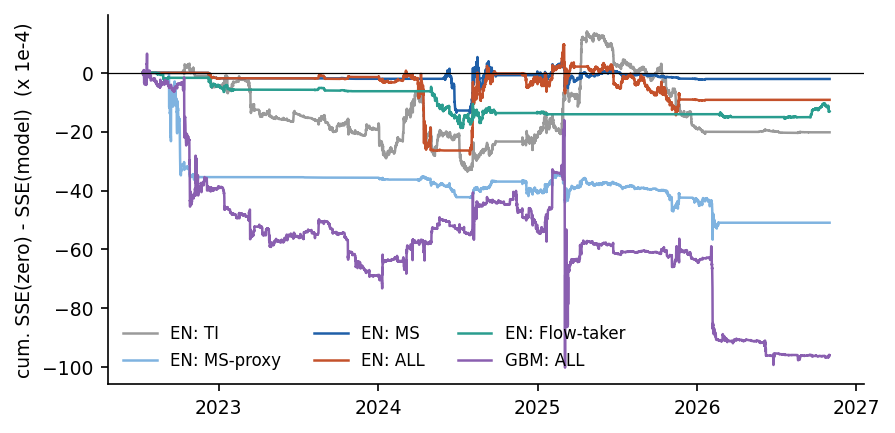
\includegraphics[width=0.8\textwidth]{fig_cum_sse.png}
\caption{Cumulative squared-error difference between the zero forecast and each model, BTC/USDT
four-hour returns. A rising line means the model is more accurate than the zero forecast.}
\label{fig:cumsse}
\end{figure}

\subsection{Incremental information}

\begin{table}[t]
\centering\caption{Incremental predictive information, BTC/USDT}\label{tab:incremental}
\resizebox{\textwidth}{!}{\begin{tabular}{llcrrrrr}
\toprule
Model & Benchmark & Nested & $R^2_{OOS}$ rel.\ (\%) & CW $t$ & CW $p$ & DM $t$ & DM $p$\\
\midrule
EN: ALL & EN: TI & yes & 0.030 & 2.41$^{***}$ & 0.008 & 0.33$$ & 0.741\\
EN: MS & EN: TI & yes & 0.050 & 2.85$^{***}$ & 0.002 & 0.55$$ & 0.585\\
EN: MS & EN: MS$_{\text{proxy}}$ & yes & 0.133 & 2.59$^{***}$ & 0.005 & 1.53$$ & 0.125\\
EN: MS$_{\text{proxy}}$ & EN: TI & yes & \ensuremath{-}0.084 & 1.49$^{*}$ & 0.068 & \ensuremath{-}0.71$$ & 0.476\\
GBM: ALL & EN: TI & yes & \ensuremath{-}0.207 & 1.73$^{**}$ & 0.042 & \ensuremath{-}0.88$$ & 0.378\\
EN: Flow$_{\text{taker}}$ & EN: Flow$_{\text{BVC}}$ & no & 0.045 & -- & -- & 0.97$$ & 0.332\\
\bottomrule
\end{tabular}
}
\tabnote{$R^2_{OOS}$ rel.: out-of-sample $R^2$ of the model relative to the benchmark. CW: Clark-West
test of the null that the larger model adds nothing to the nested benchmark (one-sided). DM:
Diebold-Mariano test of equal mean squared error (two-sided). The observed-flow and BVC-flow models are
not nested, so only DM is reported.}
\end{table}

Table~\ref{tab:incremental} asks whether each richer feature set improves on a simpler one. The
Clark-West test rejects the null that microstructure variables add nothing to technical indicators
($p=\BTCincMSTICWp$ for MS over TI and $p=\BTCincALLTICWp$ for ALL over TI) and that observed flow and
intrahour measures add nothing to the OHLCV proxies ($p=\BTCincMSMSproxyCWp$). In each case, however,
the realised gain in mean squared error is a few hundredths of a percent and the Diebold-Mariano test
does not reject equal accuracy. This is the pattern Clark-West is designed to detect: the larger
model's population coefficients are not all zero, but the information they carry is smaller than the
noise introduced by estimating them, so the larger model does not forecast better in practice.

The model selection inside each training window tells the same story. For the elastic net the
validation step chooses the penalty that sets every coefficient to zero in \BTCnullMSproxy{} of the
\BTCnFolds{} folds with the OHLCV proxies, \BTCnullMS{} with observed flow and intrahour measures, and
\BTCnullALL{} with all features, against \BTCnullTI{} with technical indicators alone. Most of the
time, the data prefer no forecast at all.

\subsection{A single predictor: observed flow against its proxy}

The flow models above combine five constructions and tune a penalty on a short validation block,
which may discard a weak but genuine signal. Section~\ref{sec:response} suggests a direct test: does
the current hour's observed taker imbalance, on its own, forecast returns out of sample, and does its
BVC counterpart? For each predictor we estimate a one-variable regression without intercept on the
standardised predictor in the same expanding monthly walk-forward, with purged labels and moments
from the training window only, and no tuning.

\begin{table}[t]
\centering\caption{Single-predictor out-of-sample test}\label{tab:single}
\resizebox{\textwidth}{!}{\begin{tabular}{lrrrrrrr}
\toprule
 & & & & & & \multicolumn{2}{c}{$R^2_{OOS}$ (CW $p$) by half}\\
\cmidrule(lr){7-8}Predictor & Horizon & $R^2_{OOS}$ (\%) & CW $t$ & CW $p$ & IC & first & second\\
\midrule
\multicolumn{8}{l}{\emph{BTC/USDT}}\\
Observed taker imbalance & 1h & 0.012 & 3.19$^{***}$ & 0.0007 & 0.048 & 0.009 (0.032) & 0.016 (0.005)\\
Observed taker imbalance & 2h & 0.021 & 3.80$^{***}$ & 0.0001 & 0.044 & 0.007 (0.022) & 0.038 (0.001)\\
Observed taker imbalance & 4h & 0.016 & 2.62$^{***}$ & 0.0044 & 0.033 & 0.003 (0.233) & 0.032 (0.006)\\
BVC imbalance (1h bars) & 1h & \ensuremath{-}0.001 & 0.74$$ & 0.2286 & 0.030 & 0.007 (0.183) & \ensuremath{-}0.011 (0.370)\\
BVC imbalance (1h bars) & 2h & \ensuremath{-}0.007 & \ensuremath{-}0.56$$ & 0.7119 & 0.015 & \ensuremath{-}0.010 (0.848) & \ensuremath{-}0.004 (0.489)\\
BVC imbalance (1h bars) & 4h & \ensuremath{-}0.008 & \ensuremath{-}0.35$$ & 0.6353 & \ensuremath{-}0.034 & \ensuremath{-}0.007 (0.484) & \ensuremath{-}0.010 (0.836)\\
BVC imbalance (1m bars) & 1h & 0.014 & 2.39$^{***}$ & 0.0085 & 0.060 & 0.027 (0.015) & 0.000 (0.111)\\
BVC imbalance (1m bars) & 2h & 0.017 & 2.55$^{***}$ & 0.0053 & 0.054 & 0.023 (0.020) & 0.009 (0.062)\\
BVC imbalance (1m bars) & 4h & 0.002 & 1.04$$ & 0.1498 & 0.038 & \ensuremath{-}0.001 (0.319) & 0.005 (0.170)\\
\multicolumn{8}{l}{\emph{ETH/USDT}}\\
Observed taker imbalance & 1h & \ensuremath{-}0.013 & 0.63$$ & 0.2652 & \ensuremath{-}0.035 & \ensuremath{-}0.025 (0.227) & \ensuremath{-}0.003 (0.911)\\
Observed taker imbalance & 2h & \ensuremath{-}0.006 & 0.14$$ & 0.4443 & 0.002 & \ensuremath{-}0.018 (0.616) & 0.004 (0.198)\\
Observed taker imbalance & 4h & \ensuremath{-}0.015 & \ensuremath{-}0.69$$ & 0.7560 & \ensuremath{-}0.016 & \ensuremath{-}0.031 (0.772) & \ensuremath{-}0.002 (0.499)\\
BVC imbalance (1h bars) & 1h & \ensuremath{-}0.006 & 0.42$$ & 0.3383 & \ensuremath{-}0.040 & \ensuremath{-}0.023 (0.448) & 0.008 (0.127)\\
BVC imbalance (1h bars) & 2h & \ensuremath{-}0.004 & 0.41$$ & 0.3405 & \ensuremath{-}0.043 & \ensuremath{-}0.005 (0.358) & \ensuremath{-}0.004 (0.423)\\
BVC imbalance (1h bars) & 4h & 0.009 & 1.20$$ & 0.1151 & \ensuremath{-}0.026 & \ensuremath{-}0.011 (0.620) & 0.025 (0.063)\\
BVC imbalance (1m bars) & 1h & \ensuremath{-}0.005 & \ensuremath{-}0.12$$ & 0.5462 & \ensuremath{-}0.018 & \ensuremath{-}0.011 (0.612) & 0.001 (0.373)\\
BVC imbalance (1m bars) & 2h & \ensuremath{-}0.005 & \ensuremath{-}0.54$$ & 0.7052 & 0.023 & \ensuremath{-}0.007 (0.733) & \ensuremath{-}0.003 (0.562)\\
BVC imbalance (1m bars) & 4h & \ensuremath{-}0.006 & \ensuremath{-}1.19$$ & 0.8829 & 0.013 & \ensuremath{-}0.010 (0.850) & \ensuremath{-}0.004 (0.725)\\
\bottomrule
\end{tabular}
}
\tabnote{One-variable expanding-window regression, re-estimated monthly with purged labels; the
coefficient is learned from past data only. $R^2_{OOS}$ against the zero forecast; CW: Clark-West
test against zero (one-sided); IC: Spearman correlation of forecast and outcome. The last two columns
split the out-of-sample period into halves.}
\end{table}

Table~\ref{tab:single} gives a clean contrast for BTC. Observed taker imbalance has a positive
out-of-sample $R^2$ at every horizon, \BTCspRtwo\% at two hours with a Clark-West $p$-value of
\BTCspPtwo{} and an information coefficient of \BTCspICtwo. The result holds in both halves of the
test period (\BTCspRAtwo\% with $p=\BTCspPAtwo$ in the first and \BTCspRBtwo\% with $p=\BTCspPBtwo$ in
the second). Hourly BVC imbalance has a negative out-of-sample $R^2$ at every horizon and no
significant Clark-West statistic. BVC on one-minute bars lies in between, with an out-of-sample $R^2$
of \BTCspbvcmRtwo\% at two hours ($p=\BTCspbvcmPtwo$), in line with the in-sample gradient of
Section~\ref{sec:response}. Because the coefficient is re-estimated from past data each month, the
sign of the relation is learned in real time; the predictor itself, however, was suggested by the
full-sample analysis, so the test is not pre-registered. Even a Bonferroni correction for all \nALL{}
candidate features leaves the two-hour result for observed flow significant at the 1\% level. For
ETH none of the three predictors forecasts returns, consistent with the weaker in-sample response.

\begin{table}[t]
\centering\caption{Trading on the single observed-flow forecast, two-hour holding period}\label{tab:single_trading}
\begin{tabular}{llrrrrrr}
\toprule
 & & Ann.\ ret.\ (\%) & \multicolumn{3}{c}{Sharpe at cost (bps)} & Turnover & Break-even\\
\cmidrule(lr){4-6} Asset & Rule & gross & 0 & 1 & 2 & per day & (bps)\\
\midrule
BTC/USDT & sign & 30.0 & 0.87 & \ensuremath{-}0.34 & \ensuremath{-}1.54 & 11.4 & 0.72\\
BTC/USDT & selective & 26.4 & 1.43 & 0.23 & \ensuremath{-}0.97 & 6.1 & 1.19\\
ETH/USDT & sign & 10.6 & 0.23 & \ensuremath{-}0.67 & \ensuremath{-}1.56 & 11.3 & 0.26\\
ETH/USDT & selective & 5.9 & 0.26 & \ensuremath{-}0.62 & \ensuremath{-}1.50 & 5.4 & 0.30\\
\bottomrule
\end{tabular}

\tabnote{Overlapping-sleeve rule on the out-of-sample forecast from observed taker imbalance alone
(Table~\ref{tab:single}, two-hour horizon). Sign: trade every hour in the direction of the forecast;
selective: only when $|\hat y_t|$ exceeds the 80th percentile of in-sample absolute forecasts.
Break-even: cost per unit turnover at which net profit is zero.}
\end{table}

Two lessons follow. First, the information that order flow carries about short-horizon BTC returns
is detectable out of sample when flow is measured, partly recoverable from one-minute prices, and
absent from hourly bars. Second, the multivariate elastic net that includes the same variable fails
to exploit it: with a weak signal and many correlated candidates, cross-validated shrinkage on a short
validation block usually selects the empty model. The signal is nonetheless far too small to trade.
Table~\ref{tab:single_trading} applies the overlapping-sleeve rule to the observed-flow forecast with a
two-hour holding period. Gross Sharpe ratios are \BTCstSRsign{} for the sign rule and
\BTCstSRselective{} for the selective rule, but the rules turn over their position many times a day,
and their break-even costs are \BTCstBEsign{} and \BTCstBEselective{} basis points per unit of
turnover. That is an order of magnitude below the standard fee of ten basis points, and below the
taker fees of high-volume accounts, which remain at a few basis points; a strategy that must trade
immediately on an hourly signal cannot rely on maker rebates. The predictable component is a
statistical regularity, not an exploitable strategy.

\subsection{Economic value}

\begin{table}[t]
\centering\caption{Trading performance of forecast-based rules, BTC/USDT}\label{tab:backtest}
\resizebox{\textwidth}{!}{\begin{tabular}{lrrrrrrrcr}
\toprule
& Ann.\ ret.\ (\%) & \multicolumn{3}{c}{Sharpe at cost (bps)} & Turnover & Break-even & $\alpha$ $t$ & Years & DSR\\
\cmidrule(lr){3-5} Model & gross & 0 & 2 & 5 & per day & (bps) & (HAC) & $SR>0$ & \\
\midrule
\multicolumn{10}{l}{\emph{Sign rule}}\\
EN: TI & 7.8 & 0.39 & \ensuremath{-}0.19 & \ensuremath{-}1.05 & 2.61 & 1.4 & 0.78 & 2/5 & 0.11\\
EN: MS$_{\text{proxy}}$ & \ensuremath{-}14.1 & \ensuremath{-}0.38 & \ensuremath{-}0.59 & \ensuremath{-}0.90 & 0.81 & \ensuremath{-}3.7 & \ensuremath{-}0.88 & 0/5 & 0.00\\
EN: MS & \ensuremath{-}10.9 & \ensuremath{-}0.40 & \ensuremath{-}0.64 & \ensuremath{-}1.00 & 0.75 & \ensuremath{-}3.3 & \ensuremath{-}0.83 & 1/5 & 0.00\\
EN: ALL & 35.5 & 1.24 & 0.97 & 0.55 & 1.04 & 9.0 & 2.68 & 3/5 & 0.70\\
EN: Flow$_{\text{BVC}}$ & \ensuremath{-}22.8 & \ensuremath{-}0.84 & \ensuremath{-}1.00 & \ensuremath{-}1.24 & 0.59 & \ensuremath{-}10.4 & \ensuremath{-}1.54 & 0/5 & 0.00\\
EN: Flow$_{\text{taker}}$ & \ensuremath{-}5.5 & \ensuremath{-}0.17 & \ensuremath{-}0.42 & \ensuremath{-}0.80 & 0.72 & \ensuremath{-}1.3 & \ensuremath{-}0.17 & 3/5 & 0.01\\
GBM: MS & \ensuremath{-}10.1 & \ensuremath{-}0.05 & \ensuremath{-}0.46 & \ensuremath{-}1.07 & 2.33 & \ensuremath{-}0.2 & 0.25 & 2/5 & 0.02\\
GBM: ALL & \ensuremath{-}10.7 & \ensuremath{-}0.06 & \ensuremath{-}0.38 & \ensuremath{-}0.87 & 1.85 & \ensuremath{-}0.4 & 0.46 & 3/5 & 0.02\\
\multicolumn{10}{l}{\emph{Selective rule (top quintile of |forecast|)}}\\
EN: TI & 10.9 & 0.71 & 0.34 & \ensuremath{-}0.21 & 0.83 & 3.9 & 1.51 & 4/5 & 0.28\\
EN: MS$_{\text{proxy}}$ & \ensuremath{-}7.8 & \ensuremath{-}0.47 & \ensuremath{-}0.66 & \ensuremath{-}0.93 & 0.38 & \ensuremath{-}5.1 & \ensuremath{-}1.21 & 1/5 & 0.00\\
EN: MS & 0.6 & 0.11 & \ensuremath{-}0.12 & \ensuremath{-}0.46 & 0.33 & 1.0 & 0.13 & 3/5 & 0.03\\
EN: ALL & 6.1 & 0.47 & 0.26 & \ensuremath{-}0.05 & 0.43 & 4.5 & 0.96 & 4/5 & 0.14\\
EN: Flow$_{\text{BVC}}$ & \ensuremath{-}8.4 & \ensuremath{-}0.59 & \ensuremath{-}0.75 & \ensuremath{-}0.98 & 0.29 & \ensuremath{-}7.5 & \ensuremath{-}1.02 & 1/5 & 0.00\\
EN: Flow$_{\text{taker}}$ & \ensuremath{-}4.9 & \ensuremath{-}0.45 & \ensuremath{-}0.74 & \ensuremath{-}1.17 & 0.39 & \ensuremath{-}3.2 & \ensuremath{-}0.89 & 1/5 & 0.00\\
GBM: MS & 8.9 & 0.49 & 0.26 & \ensuremath{-}0.08 & 0.71 & 4.3 & 1.03 & 2/5 & 0.15\\
GBM: ALL & \ensuremath{-}2.4 & 0.00 & \ensuremath{-}0.26 & \ensuremath{-}0.65 & 0.76 & 0.0 & 0.14 & 2/5 & 0.02\\
\midrule
Buy and hold & 34.8 & 0.87 & & & & & & & \\
\bottomrule
\end{tabular}
}
\tabnote{Overlapping-sleeve implementation with a four-hour holding period. Costs are per unit change
in position. Break-even: cost per unit turnover at which net profit is zero. $\alpha$ $t$: HAC
$t$-statistic of the intercept in a regression of gross strategy returns on BTC returns. Years
$SR>0$: calendar years with positive gross Sharpe ratio. DSR: deflated Sharpe ratio
\citep{bailey2014} across all \BTCnTrials{} model and rule combinations.}
\end{table}

Table~\ref{tab:backtest} translates the forecasts into trading rules. Before costs, most rules have
Sharpe ratios between $-1$ and $1$, and only \BTCnPosSRfive{} of the \BTCnTrials{} combinations keeps a
positive Sharpe ratio at five basis points. One combination stands out: the sign rule applied to
the full elastic net, with a gross Sharpe ratio of \BTCbestSR, a break-even cost of \BTCbestBE{}
basis points and almost no market exposure (beta \BTCbestBeta, alpha $t=\BTCbestAlphaT$). Three
diagnostics argue against reading it as evidence of a profitable signal. Its probabilistic Sharpe
ratio against zero is \BTCbestPSR, but once we account for having selected it from \BTCnTrials{}
candidates, the deflated Sharpe ratio is \BTCbestDSR, below conventional thresholds. Its Sharpe ratio
ranges from \BTCbestSRmin{} to \BTCbestSRmax{} across calendar years and is positive in \BTCbestYears{}
of them. And it is not the model with the best forecast accuracy, so its performance does not reflect
a systematic forecasting advantage. No rule has a break-even cost above \BTCmaxBE{} basis points, so a
trader paying the standard fee of ten basis points per side would have lost money with every rule.
